%-------------------------------------------------------------------------------
\section{Further optimizations}
%-------------------------------------------------------------------------------


\fs{the current writeback might be unecessary to explain, since we implement the below anyways... Perhaps merge writeback and this paragraph - the adjustments to fallback are "obvious"?}
\par \textbf{Shard Logging} When transaction execution touches multiple shards validation can incur redundant explicit logging overhead. When a Slow-Path is necessary to arrive at a logged decision on S different shards, resources are wasted. Consider an example in which $S-1$ shards attempt to log the decision Commit, while a single shard attempts to log an Abort decision. If the latter shard succeeds, the effort of the remaining shards was in vain. \fs{Moreover, logging is always bottlenecked by the slowest shard. }
The culprit of this phenomenon is the delayal of Two-Phase-Commit (2PC) until the Writeback phase. By preemptively making a 2PC decision \textbf{before} logging we can avoid this redundancy. We remark, that even when when all shards agree on a decision, this saves redundant coordination. \fs{This does not work for Atomic Broadcast! In AB, the voting only happens AFTER the tx has already been logged (i.e. the order has been durably replicated)}

Concretely, we designate \textbf{one} involved shard as \textit{logging Shard} $=$ \textit{involvedShards[TxID \% |involvedShard|]}, while all other shards remain responsible only for Voting. \changebars{}{The logging Shard can be determin via a determinsitic function over the \textit{involved Shards}. A simple load balanced solution may select $loggingS = involvedShards[TxID \% |involvedShard|]$}. \changebars{}{Figure \ref{fig:SingleShardOpt} shows a comparison and the revised structure. dont use this figure in actual paper} In order to log a decision, Phase1R Quorums \fs{aka shard votes} from all involved shards are required. We modify step 3 of the Validation protocol accordingly:

\fbox{\begin{minipage}{21em}
\textbf{Validation (3: C)}: Client waits for vote replies from all involved Shards.
\end{minipage}}
A client aggregates a per-shard decision for each shard according to the \textit{CommitQuorum} rule. If all shard-decisions are Commit, it attempts to log a Commit decision by sending $Phase2 \coloneqq (TxID, Commit, S \times \{CommitQuorum\}$ to all replicas in the designated logging Shard. If a single shard-decision is Abort, it stops waiting for other shard-decisions and attempts to log an Abort decision by instead sending $Phase2 \coloneqq (TxID, Abort, AbortQuorum)$. 

\underline{Additional subtlelties:} A client can go Fast-Path and return to the Writeback phase immediately only if Fast-Path Quorums were received for all shards. 

The remaining Validation protocol proceeds identically to the multi-shard version. Notice, that when only a single shard is involved, no adjustments were made. The Writeback phase instead, may proceed with just the single certificate from the logging Shard


The Fallback protocol is adjusted accordingly: A fallback replica need (and can) only be elected on the logging Shard, simplifying reconciliation and reducing the cost for interested clients. 
To further reduce unecessary load, a client may attempt to first inquire whether decisions exists at the logging shard (Fallback protocol step 1 \& 2), before sending $Rec-Phase1$ messages to all shards in order to gather votes itself (Fallback protocol step 1). 

\iffalse
\begin{figure*}
\begin{center}
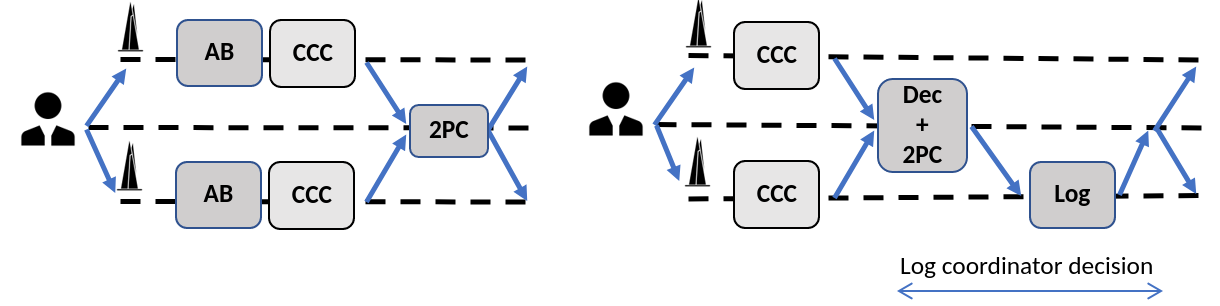
\includegraphics[width= \textwidth]{./figures/SingleShard.png}
\end{center}
\caption{Single Shard Optimization}
\label{fig:SingleShardOpt}
\end{figure*}
\fi

\par \textbf{Batching}
To amortize cryptographic overheads we introduce message batching. However, unlike leader based systems, in \sys there exists no central sequencer that may batch request. Instead, \sys implements message batching at the replicas by batching $b$ messages, generating a merkle tree \cite{merkle1987digital}, and signing only the root hash, thus reducing signing overheads from $O(b)$ to $O(1)$ per batch. The merkle hash tree allows replicas to respond to individual clients by including only the single client-addressed message and $log(b)$ additional hashes. We note, that since replicas receive requests out of order, their batches are not consistent. Consequently, a client must aggregate hashes and signatures from different merkle trees to forward as proofs (Phase2 and Writeback messages include $O(n)$ signatures and hashes) .
In order to reduce verification overheads from $O(n*b)$ to $O(n)$, replicas cache previously verified signatures by storing a mapping from signature to merkle hash roots. For following message verifications, a replica can omit de-computing the signature, and must only re-compute and compare the merkle root based on the hashes included in the proof.

\iffalse
- amortize signature cost
- unlike leader based, there is not an obvious sequencer to batch
- instead we batch signature generation at replica. Because they can be out of order these batches are different. Also do not want to send the whole batch (b* hashes) to every client. Instead we use a merkle tree and send only the root sig + log(b) hashes. (this means that we had to do 2*b hashes during signature gen, but we only do b*log(b) hashes at generation instead of b*b. OR: could send whole batch of  messages --> huge message + hashing cost..
- Cache already validated signatures at replicas and only recompute the hash to see whether it matches. This reduces verification by a factor of b (effectively only verifying for the first message from the batch).
\fi

\par Other non impelmented opts: in TR.